
\section{ping}

\subsection{Скриншоты}

\begin{center}

    \includegraphics[width=\textwidth]{screenshots/ping_1000_request_1}

    \includegraphics[width=\textwidth]{screenshots/ping_1000_request_2}

    \includegraphics[width=\textwidth]{screenshots/ping_1000_response_1}

    \includegraphics[width=\textwidth]{screenshots/ping_1000_response_2}

    \includegraphics[width=\textwidth]{screenshots/ping_2000_request_1}

    \includegraphics[width=\textwidth]{screenshots/ping_2000_request_2}

    \includegraphics[width=\textwidth]{screenshots/ping_2000_request_3}

    \includegraphics[width=\textwidth]{screenshots/ping_2000_response_1}

    \includegraphics[width=\textwidth]{screenshots/ping_2000_response_2}

    \includegraphics[width=\textwidth]{screenshots/ping_2000_response_3}

\end{center}

\subsection{Ответы на вопросы}
\subsubsection{}
Фрагментация исходного пакета начинается с размера более 1480 байт (включая заголовки).

\subsubsection{}
На это указывает флаг More Fragments IP-фрагмента.
IP-фрагменты собираются в одно сообщение с помощью полей Identification и Fragment Offset.

\subsubsection{}
Такое количество фрагментов, чтобы в них поместилось (размер сообщения + 8) байт,
по 1480 байт в одном фрагменте. 8 байт -- на заголовок ICMP.

\subsubsection{}
\begin{center}
    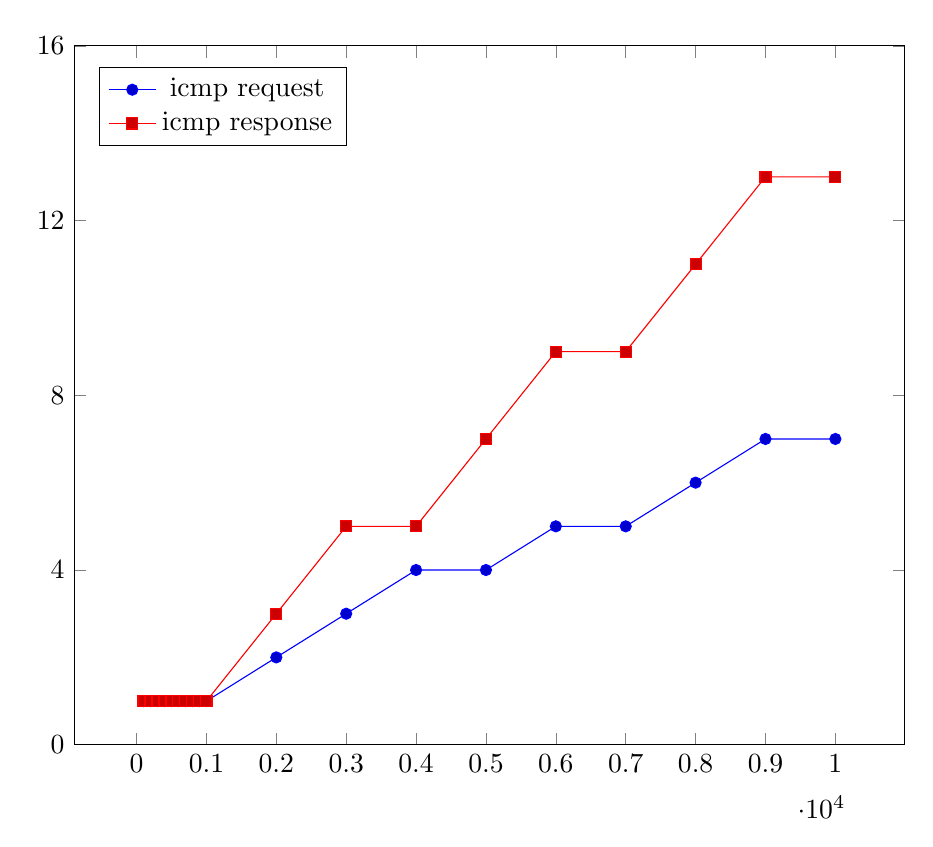
\begin{tikzpicture}
        \begin{axis}[width=\textwidth,
                ymin=0,ymax=16,
%                xtick={0,100,200,300,400,500,600,700,800,900,1000,2000,3000,4000,5000,6000,7000,8000,9000,10000},
                ytick={0,4,8,12,16},
                legend pos=north west]
            \addplot coordinates {
                (100, 1)
                (200, 1)
                (300, 1)
                (400, 1)
                (500, 1)
                (600, 1)
                (700, 1)
                (800, 1)
                (900, 1)
                (1000, 1)
                (2000, 2)
                (3000, 3)
                (4000, 4)
                (5000, 4)
                (6000, 5)
                (7000, 5)
                (8000, 6)
                (9000, 7)
                (10000, 7)
            };
            \addplot coordinates {
                (100, 1)
                (200, 1)
                (300, 1)
                (400, 1)
                (500, 1)
                (600, 1)
                (700, 1)
                (800, 1)
                (900, 1)
                (1000, 1)
                (2000, 3)
                (3000, 5)
                (4000, 5)
                (5000, 7)
                (6000, 9)
                (7000, 9)
                (8000, 11)
                (9000, 13)
                (10000, 13)
            };
            \legend{icmp request,icmp response};
        \end{axis}
    \end{tikzpicture}
\end{center}

\subsubsection{}
С помощью аргумента \texttt{-i <новый TTL>}
(при этом в ответе TTL будет таким, какой указывает адресат, поэтому отображаться изменение не будет).

\subsubsection{}
Данные сообщения об ошибке содержат копию заголовков и как минимум первые 8 байт данных провалившегося запроса.
В остальных случаях запрос содержит случайные данные, а ответ --- копию данных запроса.
